\documentclass[a4paper,12pt]{article}
\usepackage[noabs,notoc]{HaotianReport}

\title{图片HSL空间色彩分析}
\author{刘昊天}
\authorinfo{电博181班, 2018310648}
\runninghead{数据可视化课程第一次作业}
\studytime{2019年04月}

\begin{document}
    \maketitle
    %\newpage
    \part{简答题回答}
    \section{小提琴图相关问答}
    \section{圆环设计相关问答}
    \part{编程题目说明}
    \section{概述}
    本程序主体是基于D3.js(或称D3)开发的。选择D3,一方面是由于JavaScript广泛应用于前端设计,在"轻量时代"更适合开发移动编写的应用程序;另一方面则是考虑到后续各问的可视化任务高度定制化,故应采用较为底层的绘制工具。D3全称是Data-Driven Document,即"数据驱动的文档",是一个用于数据可视化的JavaScript程序包,采用BSD-3开源协议托管于Github上。很多著名的JavaScript可视化工具,都是基于D3开发的。

    另外,本程序将各个可视化任务打包,统一在Web前端进行呈现,称为Colorana(意味Color Analysis),实现图片在HSL空间上的色彩分析。这部分采用了React.js+Material-ui的技术路线,二者均为开源程序。

    作业的成果Colorana托管在Netlify平台,地址为\url{https://color.nogeek.top}。由于前端的设计并非重点,因此该网站仅保证对Chrome的支持,且未对移动端进行针对性适配。本程序将在学期结束后以MIT协议开源。

    \begin{figure}[htbp]
      \centering
      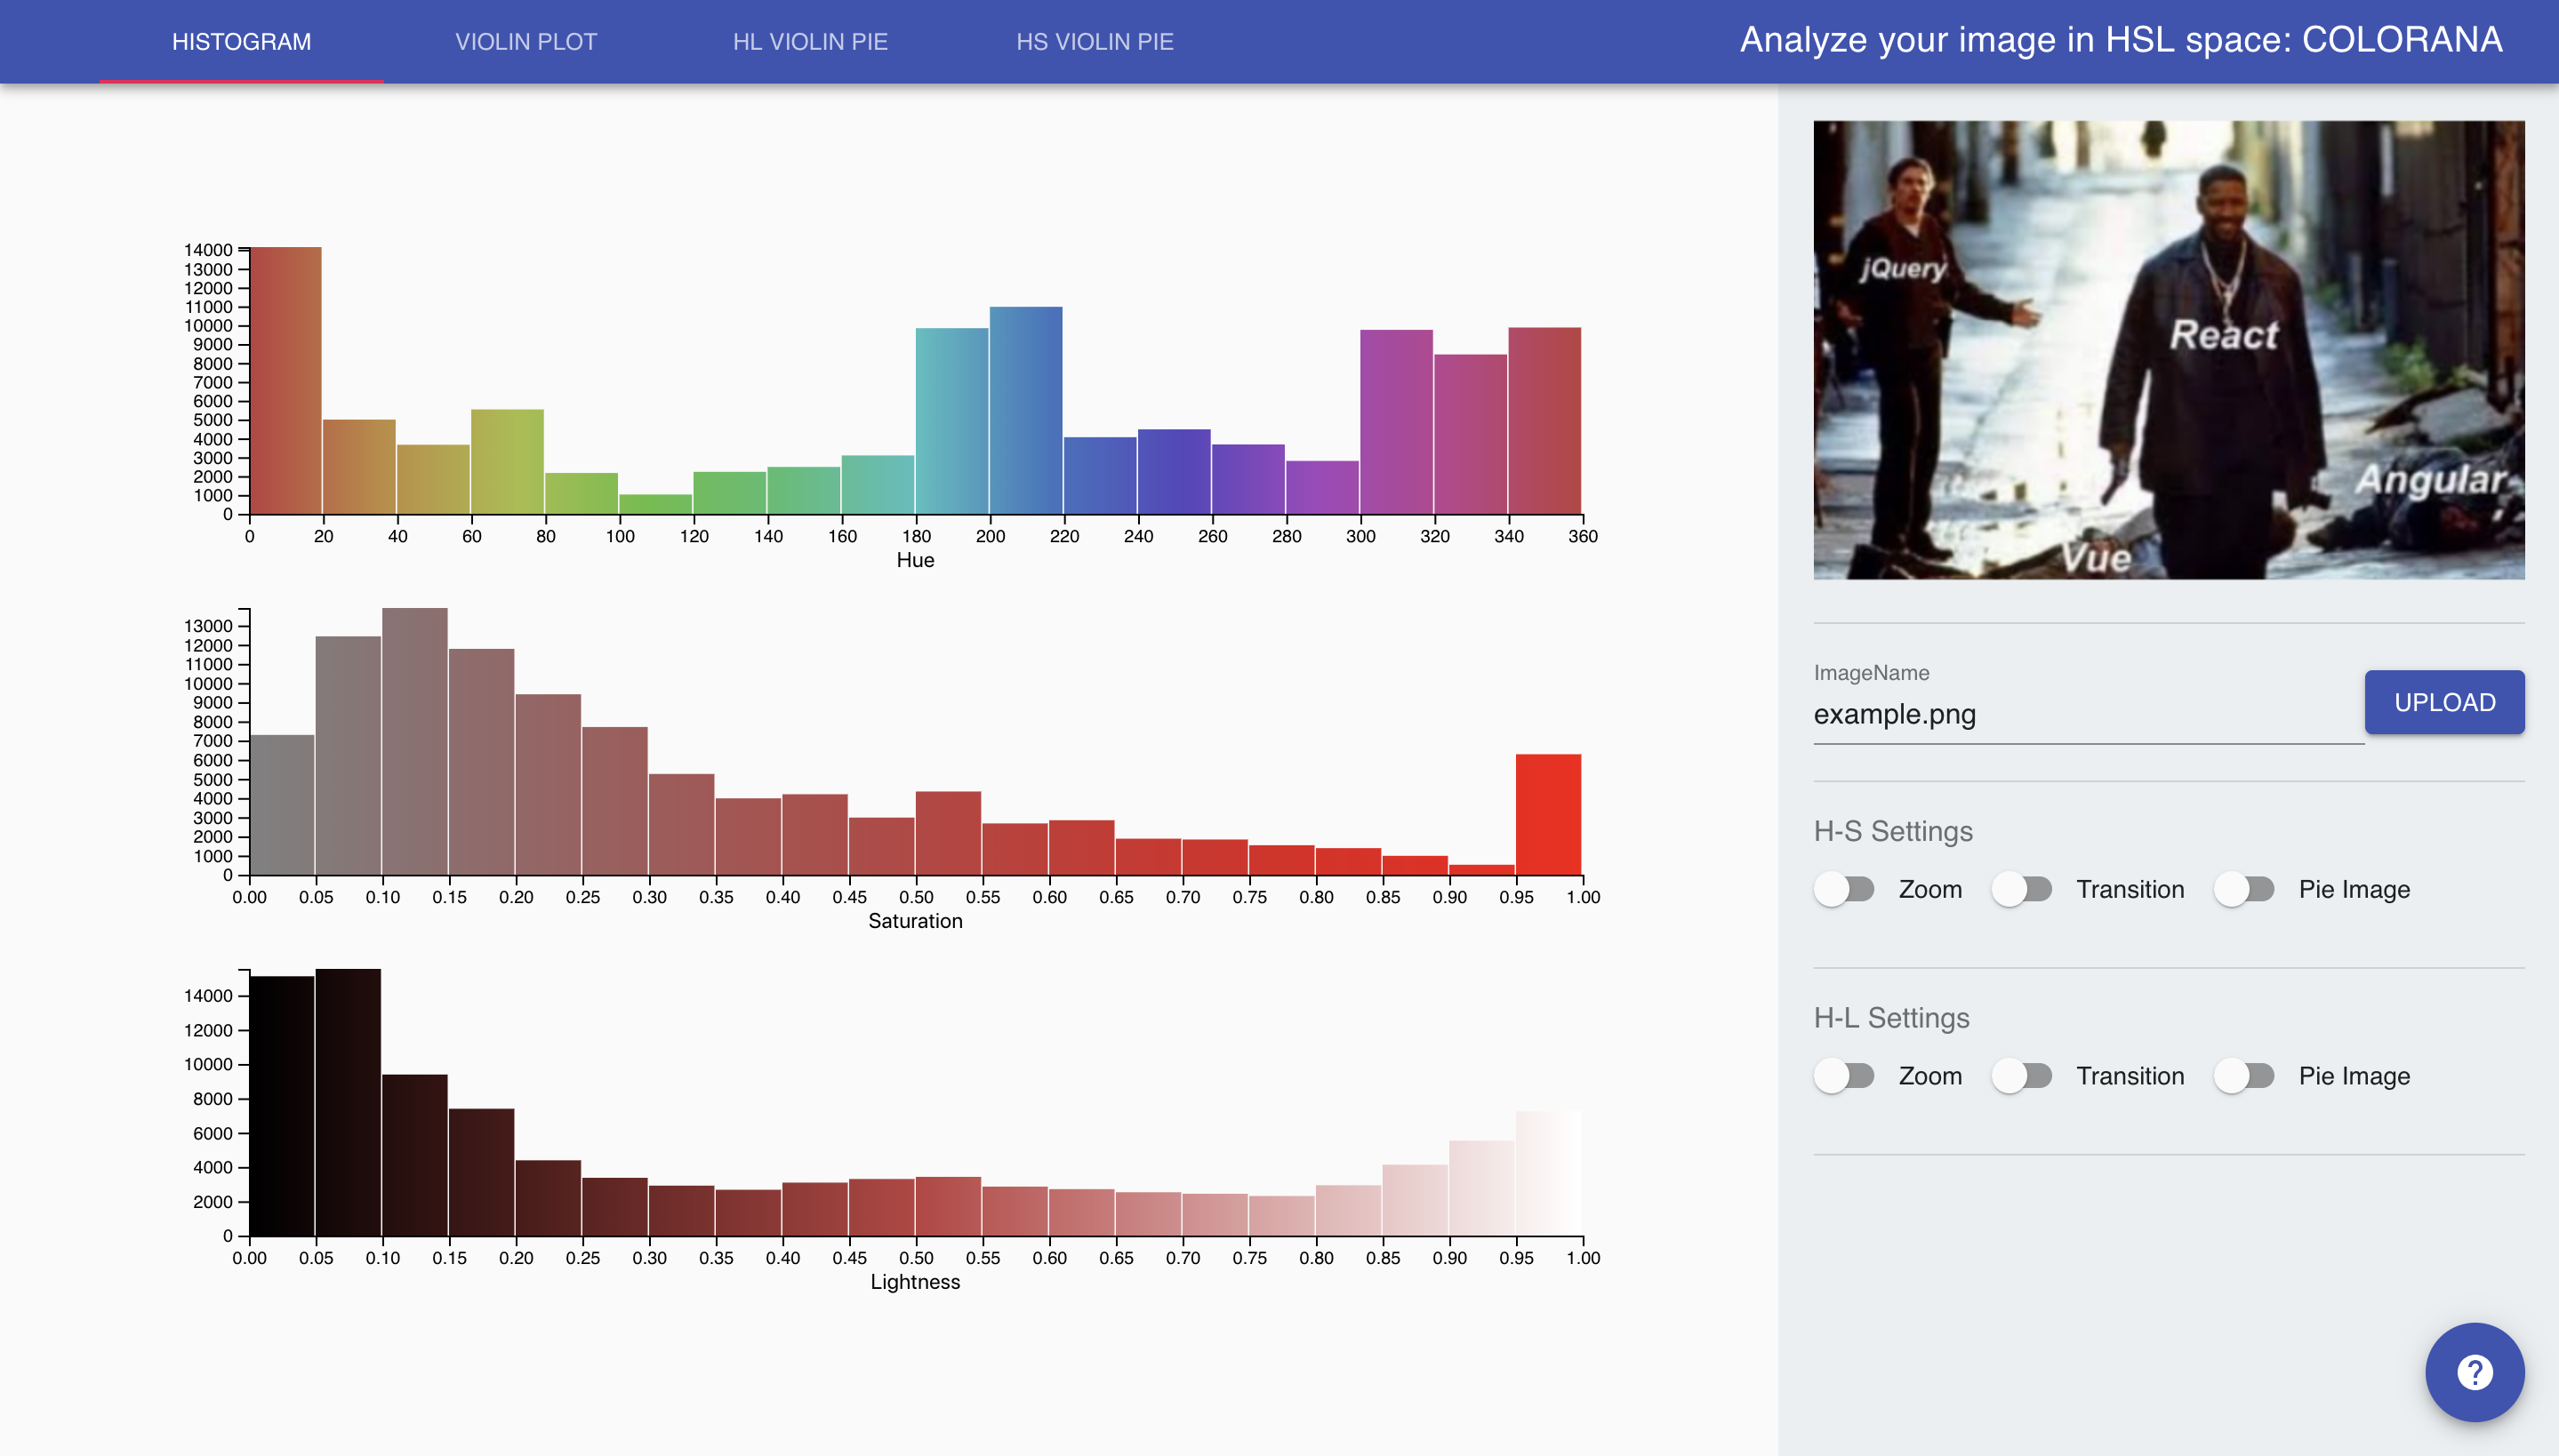
\includegraphics[width=0.9\linewidth]{frontend}
      \caption{程序前端呈现}
      \label{fig:frontend}
    \end{figure}
    \section{直方图绘制}
    \begin{figure}[htbp]
      \centering
      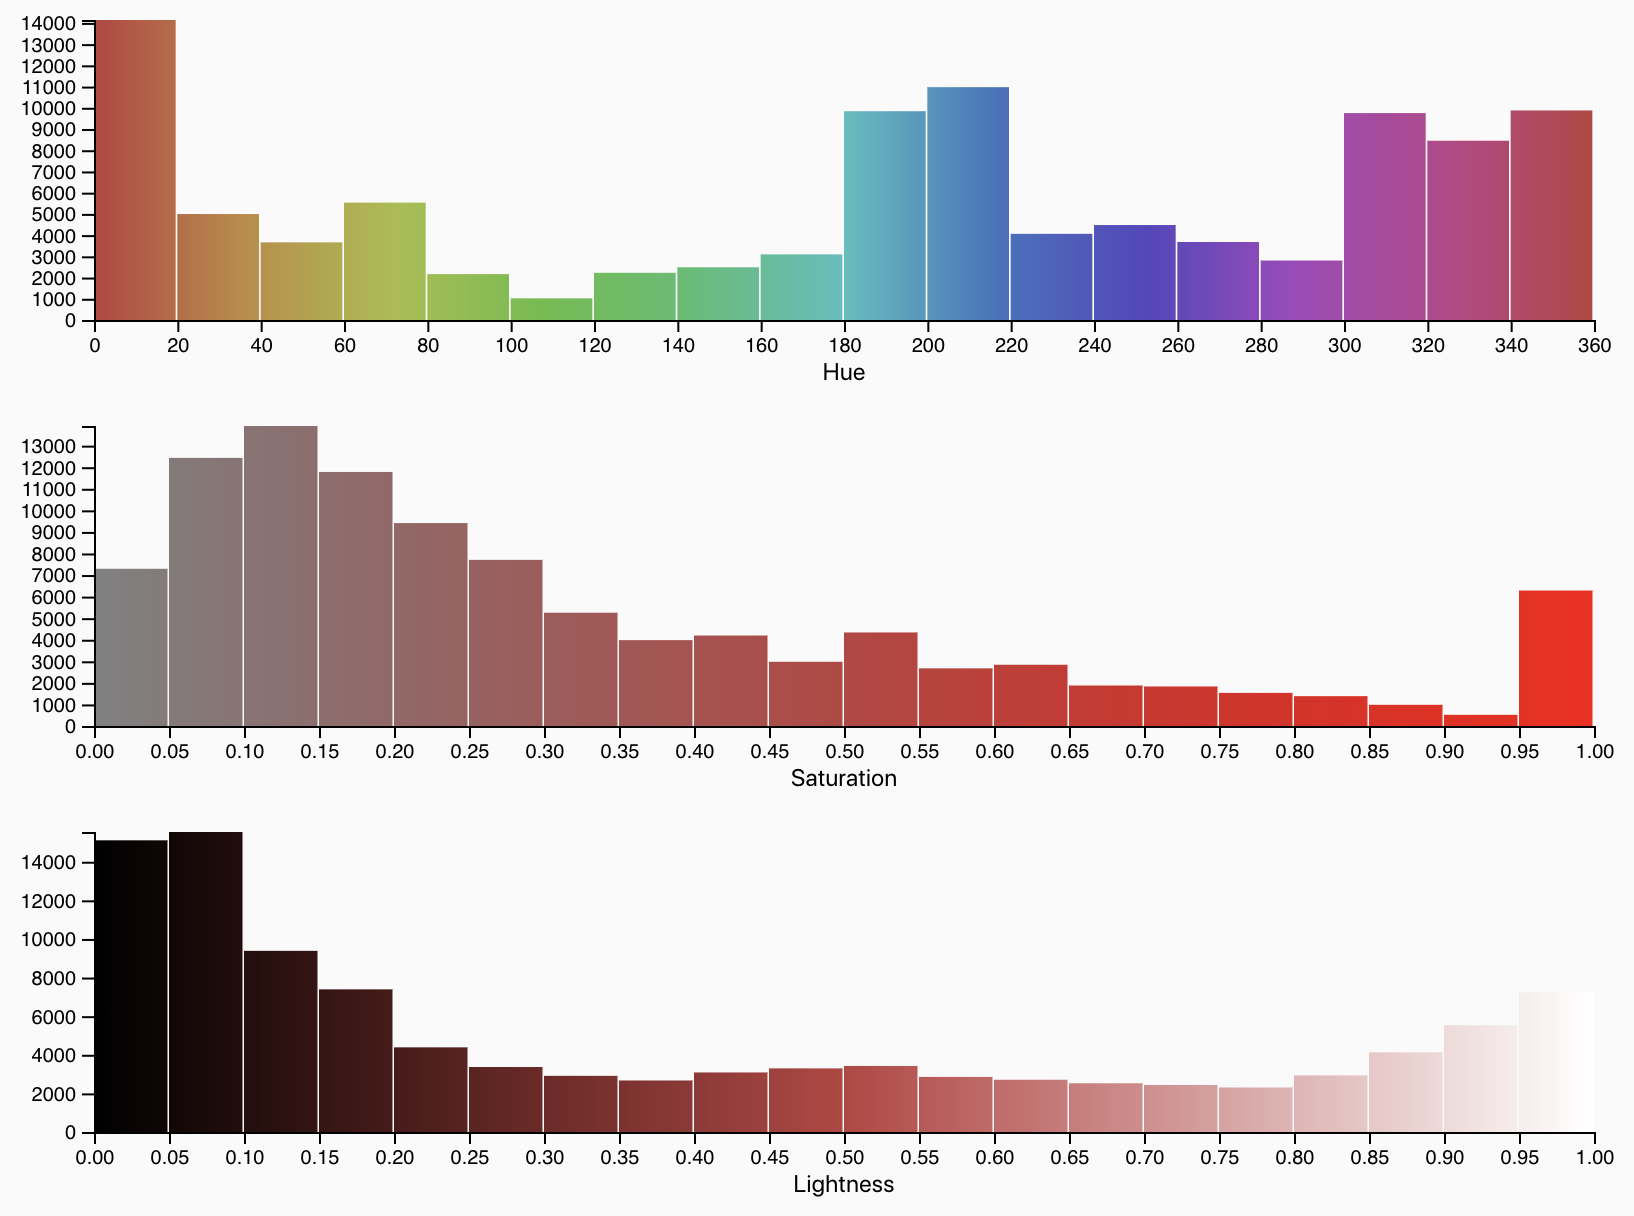
\includegraphics[width=0.9\linewidth]{histogram}
      \caption{HSL直方图绘制}
      \label{fig:histogram}
    \end{figure}

    \section{小提琴图绘制}
    \section{径向小提琴图绘制}
    \section{动画小提琴图绘制}



    \label{applastpage}
    \newpage
    \bibliography{report}
    \bibliographystyle{unsrt}
\iffalse
\begin{itemize}[noitemsep,topsep=0pt]
%no white space
\end{itemize}
\begin{enumerate}[label=\Roman{*}.,noitemsep,topsep=0pt]
%use upper case roman
\end{enumerate}
\begin{multicols}{2}
%two columns
\end{multicols}
\fi
\end{document}
